%%%%%%%%%%%%%%%%%%%%%%%%%%%%%%%%%%%%%%%%%%%%%%%%%%%%%%%%%%%%%%%%%%%%%%%%%%%%%%%%
\newpage
\section{Introduction}
\label{ch:intro}

The goal of this chapter is to describe the \emph{perspective} taken by these
notes. This perspective guides our exploration of cryptography in both overt and
subtle ways, and I think it's worth dwelling on for a bit --- successful
scholars should necessarily be introspective about why they approach problems in
certain ways, and me writing this down is such an exercise for myself. 
 
%\paragraph{The many facets of cryptography.} Cryptography, the science of secret
%writing, is a rich subject. One can approach it from historical, 
%political, philosophical or theoretical perspectives. Each provides a rich avenue
%for exploration, and every one has inspired many generations of scholars. 
%Indeed, while I greatly enjoy thinking about the cryptographic research landscape from
%the lens so elegantly crafted by Kuhn,\footnote{If you have not read the
%Structure of Scientific Revolutions, I strongly recommend it.} such philosophy will not be
%our primary focus beyond this introductory material.

Our focus will be on cryptography as a \emph{tool} for securing contemporary and
future information systems. Being in the digital age, this means
computers and their associated communication networks. One tension 
we will face is how much of contemporary technology must we consider to
build good cryptography, the details of which change rather rapidly, versus a 
more mathematical abstraction that has longer staying power. We will endeavor to
strike a balance, building lasting abstractions born out of contemporary
technology issus. 


\paragraph{Classical and modern cryptography.} A frequently espoused
viewpoint is that one can divide between modern cryptography and
classical cryptography. The tipping point 
being perhaps the seminal work of Shannon in the
1940s~\cite{shannon1949communication}, or that of Goldwasser
and Micali~\cite{shafi1984probabilistic} (and their
contemporaries) or Dolev and Yao~\cite{dolev1983security}  in the 1980s. In either case the idea is that these works
introduced a key new element into cryptography: proofs of security.
Previous to these works, in classical cryptography, one built cryptographic
algorithms and protocols and informal arguments of their security, for some
often vague notion of security. Indeed early works talk about the inability to 
recover a message from a ciphertext without the decryption key, without really
specifying what are the characteristics of these messages, how keys are chosen,
and more. 

Shannon in his work provided a beautiful mathematical definition of security for
symmetric (or secret key) encryption, called perfect secrecy. Roughly it states
that given a ciphertext, the probability, taken over the choice of secret key,
that it is an encryption of any message is the same. It's simple to state and
intuitive, and provides seemingly the best possible security, hence the name. In
the 1980s two different viewpoints emerged. On one hand, following Goldwasser
and Micali, arose the view that we should take into account computational
complexity. Roughly stated for Shannon's symmetric encryption setting, we should
only care that no computationally efficient adversary can learn something about
messages given ciphertexts.  Computational efficiency was measured in asymptotic
terms, though Bellare and Rogaway pioneered a concrete security approach that
enabled a more granular accounting of computational resources in a sequence of
papers in the 1990s~\cite{bellare1994security}.  This line of work built off techniques from
computational complexity theory, including the use of manually written
reductions relating difficulty of an adversary breaking a scheme to the
difficulty of breaking some underlying believed-to-be computationally hard
problem.  In parallel a body of work built off Dolev and Yao's ideas, in which
proofs that dispensed with computational complexity, primarily treated lower
level primitives as ``perfect'' symbolic operations, and utilized techniques
from the theory of programming languages. It is of historical and sociological
interest that the two threads of research built two largely disjoint academic communities
(researchers, conference venues, etc.).

Taken together, the use of precise security
goals stated in mathematical language and frameworks for proving schemes
protocols secure represents a big shift in the way cryptography has been
analyzed.
In the last 40 years especially, we have seen a blossoming of public
work in cryptography focused on proving security, with a vibrant academic
community focusing on it. 

%Some people refer to the shift to using proofs as 
%having moved cryptography from an art to a science.
%I have always found this characterization strange. While opinions differ exactly 
%on what is science, a dictionary definition just searched on the Internet is 
%\begin{quote}
%\emph{the intellectual and practical activity encompassing the systematic study of the
%structure and behavior of the physical and natural world through observation and
%experiment.}
%\end{quote}
%%If one goes
%%back and reads early ``artistic'' works on cryptography, one finds a lot of
%%experimentation, observation, and data analysis.\tnote{Confirm this with some
%%examples}
%Reading the landmark papers of contemporary ``provable security'' cryptography,
%one notes a conspicuous absence of observation and experimentation.  I suppose
%one could instead redefine science to include this kind of mathematical
%cryptography, but this would seems to me to be the tail wagging the dog. What's
%more, barring modern cryptography papers with their elegant theorem statements
%and clever proofs from being considered art is cruel. 

%From our utilitarian viewpoint, the important question is not how to best
%pigeonhole academic efforts as science, math, or engineering, but rather to ask
%whether, and to what extent, they help us build secure cryptographic tools.  

\paragraph{The ground truth of (in)security.} Security is inherently normative
and context-dependent. We will take a pragmatic viewpoint on evaluating
security: Are real attacks being foiled? By real attacks, I mean evidenced cases
in which actors have sought to, or more likely, achieved harm against some
computing system.  We will have to use our normative judgement on what is harm,
but the point here is that, for the researcher, we will attempt to steer our
design and evaluation of cryptography towards practical security issues.
Cryptosystem A will dominate cryposystem B if we can point to real attacks that
it foils while cryptosystem B only provides some hypothetical improvements. 
Evidence of real attacks can be garnered through word-of-mouth discussions with
practitioners, or even research into attackers motives and means.  

Unfortunately judging efficacy is not yet formulaic, and coming up with rigorous ways
to predict whether cryptographic designs prevent attacks represents an
opportunity area for much future research. 
%This may sound strange given all the amazing tools we have developed
%to aid our design of cryptography, but at least it provides solace in that
%researchers are going to be in demand for many generations to come.


\paragraph{Methodoligical regimes.} Towards better predictions, we want
principled approaches. 
One can roughly group together various methodological regimes cryptographers use
to evaluate whether a cryptographic design will resist attack.  
Examples include: 
\begin{newitemize}
\item  Cryptanalysis (here I mean the study of blockciphers, hash functions,
number-theoretic primitives, and other low-level cryptographic primitives)
\item  Developing attacks (against algorithms and protocols, or implementations of them)
\item  Algorithm verification (such as Dolev-Yao type
analyses) or even software verification
\item  Reduction-based analysis (very often called provable security)
\item  Empiricism (understanding cryptographic system behavior in the real world)
\item  User studies (to determine if cryptographic systems easy implement and use securely) 
\end{newitemize}
Each regime offers instruments for scrutiny of cryptography, and they
each have their strengths and weaknesses. If one wants to understand how
attackers can exploit an implementation of a cryptosystem, it's probably not best to start with
verification or reduction-based security --- start by playing the role of an attacker and applying your experience
and ingenuity.  On the other hand, if you want to rule out attacks that violate
the lower-level structure of the cryptographic algorithms, then using
reduction-based analysis to show that the design appears to be secure as long as
some underlying hard problem remains so. If you want to understand if problems
are hard, you're back to the body of cryptanalytic work attempting to build fast algorithms
for factoring, discrete log, or finding collisions in hash functions.
If you have an interactive protocol for which manual analysis exceeds typical expert human capacity,
then you should probably start looking towards symbolic analysis tools. 

In line with our utilitarian viewpoint, you picked the right tool not because of
success measured by aesthetic concerns such as the cleverness of a demonstrated
attack, the elegance of a reduction, or improvements in type theory, but rather
because it helped you build a system resisting the types of attacks seen in
practice. To really gain confidence should most typically use a combination of
methodological regimes to gain confidence in a design, such as was used in a
large effort for the recent TLS 1.3 specification, which used a combination of
almost all the regimes above.  A sophisticated cryptographer will of course,
appreciate and try to understand the gaps between different methodological
regimes -- the attacks that they don't, in aggregate, rule out.  


Unfortunately, I don't know much about approaches --- there
are only so many hours in one's life --- and so many will sadly only get cursory
discussion.  I will focus a lot on reduction-based analysis in the
concrete-security tradition,  developing attacks, and empiricism, the topics for
which I have some experience. They will serve as good examples to understand the
rough boundaries between different methodological regimes and the fascinating
issues that arises at those boundaries. 


\paragraph{The power and pitfalls of abstraction.}  A key element to any
security analysis is abstraction, and security analyses use abstraction
aggressively to ensure analytical tractability. Abstractions in our context is an exercise
in \emph{modeling} of cryptographic settings.  For example, we will spend a lot
of time developing security games that capture desirable security properties for
cryptographic algorithms. 

Modeling is hard. The reason is we must simultaneously balance the need for
simplicity of an abstraction with the danger of omitting security-critical
details. As a ready example, almost all of our modeling will not countenance
side-channel attacks such as those emanating from analyzing power traces or
microarchitectural nuances.  Would we be better off with models that do try to
take these into account?  In most cases the seeming answer is `no', because the
models would become too complicated to allow useful analysis. 


We therefore advocate an iterative approach to modeling that
roughly goes as follows:
\begin{newenum}
\item Identify normative security concerns. Or put more simply: what attacks do we believe
people care about preventing?  
%
\item Develop one or more cryptographic security models that (hopefully) speak to these
attacks. Analyze different models formally by comparing them. Develop cryptographic
systems that we can show analytically are secure in the model.
%
\item Return to normative security goals. Can we break our proposed schemes
in some normatively damaging way?  
\end{newenum} 
I use the term normative here to indicate the fact that, ultimately, security
is a social construct and we are driven by people's desires. We won't, in this
class, put a significant amount of attention on tools for wading through the ethical and
sociological questions of how we should guide our normative concerns --- that
requires philosophy.\footnote{One might read Rogaway's paper on this topic for
further pointers
\url{http://web.cs.ucdavis.edu/~rogaway/papers/moral-fn.pdf}.}  
That said, we can identify interesting security concerns via intuition,
experience, and keeping tabs on socially important topics. My favorite approach
is to pay close attention to what problems practitioners are facing --- what attacks have
arisen in practice that cryptography might solve? Develping the ability to
identify such opportunities can be a good way to build a career of impactful
research. 

Once normative concerns are identified, we can attend to how we can address them
as rigorously as possible. Here we come up with security models, often called
security definitions. We will build off the tradition of
what's called provable security cryptography that provides definitions in the way of
probabilistic experiments. We will discuss how to formalize in subsequent
chapters. Within these abstractions we will also be able to define absractions
of cryptographic tools: these are the pseudocode versions of real software or
hardware. These serve as a specification of sorts, though often these are, like
security models, woefully lacking in details from the perspective of an
implementor. A key issue will be attending to this tension between level of
detail and modeling simplicity. 

We will then show how to do various formal analyses in these abstract models.
The approach will be hand-written proofs, in a mathematical style. They will
most often be reduction-based and we will focus on ensuring, whenever possible,
that  analyses result in actionable information about the security of a proposed
cryptographic algorithm. 

We will then return to understanding limitations of what we've produced by way
of developing attacks against normative security goals. Often we can iteratively
develop formal models to attend to these attacks, helping suss out subtleties
missed in earlier iterations. However, at some point we expect that more
modeling will have diminishing returns: either the normative attacks can't be
found or seem more
easily dispensed with via informal guidance (e.g., use padding when necessary to
obscure lengths, use constant-time code).

Given our utilitarian viewpoint, we will want, throughout, to attend to practicality: 
Are the cryptographic algorithms
we arrive at reasonable for use? Are they fast enough for practice? 
Will they be fragile to implement? If the answers are no, that doesn't
necessarily mean that some effort should be discarded --- it may be fascinating
theory that has value for the future. But we should at least 
be able to articulate how far from practical some proposal is, and why. This
often requires experimentation, measurement, and dealing with often messy 
issues such as legacy requirements or psychological acceptability by developers.

The viewpoints above may stand in stark contrast to the rhetoric of provable
security more often used in modern treatments of cryptography. What people refer
to as provable security is just the step (2) above, but I try to avoid this
terminology because I think (and experience indicates) that it oversells and may
often under-deliver. Proofs can have errors. Models can become so complex they
have limited analytical utility and using them leads to mistakes or overly
complex protocols that are hard to implement.  In any case, while for
theoreticians provable security is a meaningful term, for cryptography meant to
be secure in practice, it risks being misleading. Nothing is so black-and-white
in practice.

\begin{wrapfigure}{r}{3in}
\center
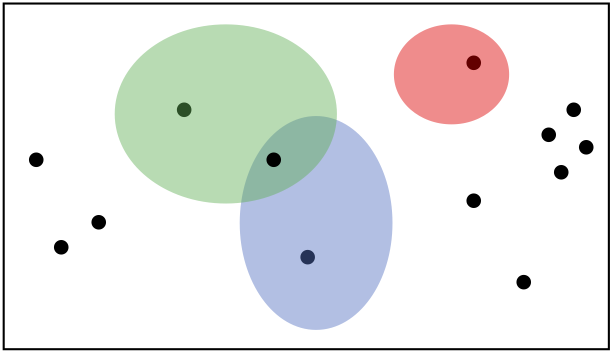
\includegraphics[width=2.5in]{venndiagram-cropped.png}
\caption{The universe of possible attacks against a cryptographic scheme or
protocol.} 
\label{fig:venndiagram}
\end{wrapfigure}


This is not to say that theory, modeling, and formal analysis aren't critical to
applied cryptography. Most obviously we will be building off the deep literature
from theoretical cryptography, and without that theory we would be lost. More
directly, theory provides us powerful tools to help us rule out large
classes of attacks for deployed schemes, that complement and strengthen the one-at-a-time
approach of simple attack-driven investigations. 
One can visualize this process for a particular
scheme as shown in \figref{fig:venndiagram}, which means to depict the universe of all
possible attacks and those attacks covered by different analysis approaches. Each point in
this universe represents an implementable attack against an instantiation 
of the system, which may or may not succeed, and the goal of the analyst is to rule out
the efficacy of as many such attacks as possible.  The black dots
represent one-at-a-time investigation ruling out individual attacks, the
green circle might represent formal reduction-based analyses, the blue circle
symbolic analyses, and the red circle an analysis of some class of side-channel
attacks.  Of course this is highly abstracted, but gives a sense of the
thinking: formal modeling and analysis can help rule out larger classes of
attacks, but certainly will miss things that fall outside the scope of the
model. By combining approaches in a thoughtful manner combined with normative
intuition, one achieves better coverage and can spot attack strategies that may
be more likely to work.

To make this kind of approach work, though, we must have a mastery of modeling
and formal analysis tools. Gaining that mastery is the subject of this course.





